% --- INICIO DE PLANTILLA PERSONALIZADA ---
\documentclass[oneside,11pt]{Latex/Classes/PhDthesisPSnPDF}

% --- Paquetes Originales ---
\usepackage{blindtext}
\usepackage{actuarialangle} 
\usepackage{tabularx}
\usepackage{float}
\usepackage{multirow, array}
\usepackage[usenames,dvipsnames,svgnames,table]{xcolor}
\usepackage{longtable}
\usepackage{latexsym,amsmath,amssymb,amsfonts}
\usepackage{enumitem}
\usepackage{xparse}
\usepackage{booktabs}
\usepackage[round, sort, numbers]{natbib}  
\usepackage{adjustbox}
\usepackage[utf8]{inputenc}
\usepackage{caption}
\usepackage{graphicx}
\usepackage{hyperref}
\usepackage{cleveref}

% Definición de colores
\definecolor{miblue}{RGB}{68, 114, 196}

% --- CAMBIO CRÍTICO 1: Usar \input para macros en el preámbulo ---
% \include da problemas antes del begin document. \input es seguro.
\input{Latex/Macros/MacroFile1}

% --- Definiciones de seguridad (por si la clase falla al cargar alguna variable) ---
\providecommand{\facultad}[1]{\def\lafacultad{#1}}
\providecommand{\escudofacultad}[1]{\def\elescudo{#1}}
\providecommand{\degree}[1]{\def\elgrado{#1}}
\providecommand{\director}[1]{\def\eldirector{#1}}
\providecommand{\lugar}[1]{\def\ellugar{#1}}
\providecommand{\degreedate}[1]{\def\lafecha{#1}}

% --- Configuración para bloques de código de R (Pandoc) ---

%%%%%%%%%%%%%%%%%%%%%%%%%%%%%%%%%%%%%%%%%%%%%%%%%%%%%%%%%%%%%%%%%%%%%%%%%%%%%%%%
%                         DATOS (Conectados a RMarkdown)                       %
%%%%%%%%%%%%%%%%%%%%%%%%%%%%%%%%%%%%%%%%%%%%%%%%%%%%%%%%%%%%%%%%%%%%%%%%%%%%%%%%
\title{Análisis del comportamiento de los jugadores en línea en función
de la ubicación geográfica y el género del videojuego, horas de uso y
frecuencia de sesiones}
\author{Estefani Carreño \\ Aziel González}

% Lógica para Facultad: Si la defines en el YAML la usa, si no, usa la default

\facultad{Facultad de Ciencias Económicas y Sociales \\ Escuela de
Estadistica y Ciencias Actuariales}
  \escudofacultad{Latex/Classes/Escudos/faces}

\degree{Computación I}
\director{Jesús Ochoa \\ Oliver Triveño}
\degreedate{Abril 2026} 
\lugar{Caracas}

\portadatrue 

% Metadatos PDF
\keywords{}
\subject{}

% --- CORRECCIÓN PARA PANDOC NUEVO (Imágenes) ---
\makeatletter
\providecommand{\pandocbounded}[1]{#1}
\makeatother


%%%%%%%%%%%%%%%%%%%%%%%%%%%%%%%%%%%%%%%%%%%%%%%%%%%%%
%                   DOCUMENTO                       %
%%%%%%%%%%%%%%%%%%%%%%%%%%%%%%%%%%%%%%%%%%%%%%%%%%%%%
\begin{document}

\maketitle

%%%%%%%%%%%%%%%%%%%%%%%%%%%%%%%%%%%%%%%%%%%%%%%%%%%%%
%                  PRÓLOGO                          %
%%%%%%%%%%%%%%%%%%%%%%%%%%%%%%%%%%%%%%%%%%%%%%%%%%%%%
\frontmatter

% Puedes agregar dedicatorias desde el YAML si quieres, o dejarlas fijas aquí

%%%%%%%%%%%%%%%%%%%%%%%%%%%%%%%%%%%%%%%%%%%%%%%%%%%%%
%                   ÍNDICES                         %
%%%%%%%%%%%%%%%%%%%%%%%%%%%%%%%%%%%%%%%%%%%%%%%%%%%%%
\setcounter{secnumdepth}{3}
\setcounter{tocdepth}{3}

\tableofcontents



\cleardoublepage

  \cleardoublepage       % Empieza en página derecha (estándar en tesis)
  \chapter*{Resumen}     % Crea el título "Resumen" sin numeración (Capítulo *)
  \addcontentsline{toc}{chapter}{Resumen} % (Opcional) Lo añade al índice
  
  En el presente trabajo se realiza un análisis estadístico sobre el
comportamiento de los jugadores de videojuegos. Se examina la influencia
de la ubicación geográfica y el género del juego en los patrones de
consumo, evaluando específicamente la intensidad de uso (horas totales)
y la frecuencia de sesiones semanales. El estudio aplica técnicas
estadísticas descriptivas y visualización de datos con
R.             % Aquí se pega el texto que escribiste en el YAML
  
  \cleardoublepage

%%%%%%%%%%%%%%%%%%%%%%%%%%%%%%%%%%%%%%%%%%%%%%%%%%%%%
%                   CONTENIDO (El Corazón)          %
%%%%%%%%%%%%%%%%%%%%%%%%%%%%%%%%%%%%%%%%%%%%%%%%%%%%%
\mainmatter
\def\baselinestretch{1.5}

% --- CAMBIO CRÍTICO 2: Aquí RMarkdown inyecta todo tu texto ---
\chapter*{Introducción}

La industria de los videojuegos ha dejado de ser un nicho para
convertirse en un pilar económico global. Sin embargo, el éxito de un
título no es accidental, sino el resultado de entender la compleja
interacción entre la cultura regional y las preferencias de género de
los usuarios. Para el análisis de datos, esto plantea un reto clave:
¿Cómo influyen la ubicación y el tipo de juego en la fidelidad y el
tiempo que un usuario dedica a un videojuego?

El presente trabajo realiza un análisis estadístico exhaustivo sobre el
dataset Online Gaming.csv. Mediante el uso de herramientas en R y
técnicas de visualización, se busca descomponer el comportamiento del
jugador en función de su ubicación geográfica y el género del
videojuego. Al adoptar un enfoque de corte transversal sobre una muestra
sintética, este informe transforma métricas de intensidad y frecuencia
de uso en información estratégica para la toma de decisiones en el
sector de los videojuegos.

\section*{Estructura del informe}

\begin{itemize}
  \item{En el Capítulo I, se plantea la problemática de la variabilidad en los patrones de consumo, los objetivos, las variables de estudio, y el periodo de referencia.}
  \item{En el Capítulo II, se establece el Marco Teórico, información necesaria para el informe, definiendo los conceptos estadísticos clave como esperanza matemática, correlación, necesarios para la interpretación de los datos.}
  \item{En el Capítulo III, se describe las Bases Metódicas, detallando la naturaleza sintética del dataset y su proceso de limpieza. }
  \item{El Capítulo IV presenta el Análisis de Resultados, donde se exhiben tablas y gráficos generados dinámicamente en R Markdown es interpretrandolos.}
  \item{En el Capítulo V, se exponen las Conclusiones derivadas del análisis, orientadas a la toma de decisiones basada en los datos obtenidos.}
\end{itemize}

\chapter{Planteamiento del Problema}

A pesar del enorme y constante crecimiento que ha experimentado la
industria global de los videojuegos en los últimos tiempos, existe una
necesidad de contar con estudios especializados. Estos análisis deben
centrarse en la recopilación y examen de ciertos datos específicos que
poseen la capacidad de influir de manera determinante en los patrones de
uso de los jugadores. Al respecto, se considera que el conocimiento de
los datos es esencial para ganar y mantener una ventaja competitiva, ya
que sin la capacidad de responder a tendencias de comportamiento
críticas se pierden oportunidades para atraer jugadores rentables
(Vertica, 2024).\\

Ahora bien, dentro de estas variables críticas, destacan factores como
la Ubicación de los usuarios y el tiempo de consumo que estos dedican,
siempre analizados en estrecha relación con el género de juego en
cuestión. Sobre esto, investigaciones señalan que la cultura nacional
explica una parte de la varianza en los estilos de juego (Tilburg
University, 2023) y que regiones como Norteamérica lideran el desempeño
en ventas, especialmente en géneros como Acción (Olagunju, 2026). Para
profundizar en este entendimiento, resulta fundamental abordar una serie
de interrogantes que definen la dinámica del sector:\\

\textbf{1.} ¿Cuáles son los géneros más populares en cada región y cómo
se relacionan con la intensidad y frecuencia de juego?\\

\textbf{2.} ¿Se puede establecer una relación directa entre el tiempo
total invertido y la cantidad de sesiones semanales?\\

Como consecuencia, esta fragmentación en el conocimiento existente
impide, por ejemplo, determinar si los patrones de consumo responden más
a factores culturales debido a su región o a características intrínsecas
de cada tipo de juego. Asimismo, dificulta la identificación de perfiles
de usuario basados en la intensidad de uso y su relación con la
frecuencia de acceso, parámetros que definen a grupos de jugadores
``hardcore'' vs.~``casuales'' (Kapalo et al., 2015), información crucial
para el diseño de experiencias personalizadas (ResearchGate, 2025).\\

Por tal motivo, la obtención de respuestas claras, detalladas y
fundamentadas a estas preguntas no es un mero ejercicio estadístico; es
una herramienta necesaria para alcanzar una comprensión integral del
comportamiento del mercado. Solo a través de este conocimiento, es
posible prever las reacciones de la audiencia y asegurar la efectividad
de las estrategias aplicadas a la hora de realizar el lanzamiento de un
nuevo producto.

\section{Justificación}

La relevancia de la presente investigación reside en la necesidad de
realizar un análisis de los entornos regionales durante la fase de
planeación de cualquier proyecto de software interactivo. Se observa que
el consumo de géneros específicos de videojuegos no es un fenómeno
uniforme, sino que presenta una variabilidad significativa condicionada
por factores ideológicos, culturales y geográficos propios de cada país
o continente. Esta diversificación en los patrones de uso constituye una
fuente de información de alto valor estratégico para las empresas del
sector.

Por otro lado, desde una perspectiva empresarial, la comprensión de
estas dinámicas regionales es un factor determinante para la viabilidad
económica y la sostenibilidad de las desarrolladoras. Dado que el
objetivo primordial de estas organizaciones es el lanzamiento de
productos de éxito que aseguren su permanencia en el mercado, resulta
imperativo analizar variables como la afinidad por género de juego y su
correlación directa con el tiempo de consumo por parte del usuario.

Finalmente, el estudio de estos indicadores permite establecer
proyecciones informadas sobre el desempeño comercial de un proyecto. Al
identificar qué géneros tienen mayor tracción en plazos de tiempo
determinados según la región, es posible obtener indicios tempranos
sobre el grado de aceptación y el éxito potencial que un desarrollo
podrá alcanzar en el futuro, minimizando así la incertidumbre en la toma
de decisiones.

\section{Objetivos}

\subsection{Objetivo General}

Analizar la relación entre la ubicación geográfica y la preferencia de
género de videojuego, evaluando cómo estas variables influyen en los
patrones de intensidad y frecuencia de uso de los jugadores.

\subsection{Objetivos Específicos}
\begin{itemize}
  \item{Identificar cuáles son los géneros de juego más populares en cada ubicación para establecer el contexto del mercado.}
  \item{Comparar las horas de dedicación y frecuencia de sesiones semanales entre distintos géneros de videojuegos.}
  \item{Evaluar la distribución de las horas totales de juego registradas por los usuarios para identificar niveles de dedicación.}
  \item{Verificar si existe una relación directa entre el tiempo total de juego y la frecuencia semanal.}
\end{itemize}

\section {Variables de estudio}

\begin{table}[ht]
\centering
\caption{Variables consideradas} 
\resizebox{10cm}{!} {
\begin{tabular}{cll}
  \hline
  \textbf{TIPO} & \textbf{VARIABLE} & \textbf{DESCRIPCIÓN} \\ 
  \hline
  Categórica & Game Genre & Género del videojuego \\ 
  Categórica & Location & Locación donde se jugó el videojuego (país) \\ 
  Numérica & Sessions Per Week & Cantidad de sesiones de juego a la semana \\
  Numérica & Playtime Hours & Horas totales dedicadas a jugar \\ 
   \hline
\end{tabular}
}
\end{table}

\section{Variables y Análisis}

El estudio se organiza en cuatro partes principales que permiten
entender el comportamiento del usuario desde distintas perspectivas:

\begin{itemize}
  \item{Género del videojuego y locación donde se jugó el videojuego: Cruzamos el género del videojuego con la ubicación del jugador. Esto nos permite establecer el contexto del mercado e identificar si ciertos tipos de juegos son éxitos globales o si su popularidad depende de factores culturales de cada país.}
  \item{Cantidad de sesiones de juego a la semana y horas totales dedicadas a jugar: Comparamos las horas totales de juego con la frecuencia de sesiones semanales. Este análisis revela si el jugador prefiere sesiones largas y esporádicas o accesos cortos pero frecuentes, diferenciando el comportamiento según el género del videojuego.}
  \item{Horas totales dedicadas a jugar: Analizamos la distribución de las horas de juego para clasificar a los usuarios según su compromiso.}
  \item{Cantidad de sesiones de juego a la semana y horas totales dedicadas a jugar: Verificamos si hay una relación directa entre el tiempo total y la constancia semanal. El objetivo es determinar si un aumento en las sesiones se traduce necesariamente en una mayor cantidad de horas totales, validando la consistencia del jugador.}
\end{itemize}

\section{Periodo de Referencia}

El presente trabajo utiliza el dataset Online Gaming.csv, el cual es un
conjunto de datos de naturaleza sintética diseñado para el modelado
estadístico y predictivo, suministrado por la unidad curricular. Dado
que los registros han sido generados algorítmicamente para simular
patrones de comportamiento de usuarios, el estudio prescinde de un
periodo de referencia cronológico. En su lugar, se adopta un enfoque de
corte transversal, donde el análisis se centra exclusivamente en las
correlaciones y distribuciones de las variables de consumo en un entorno
controlado y atemporal.

\chapter{Marco Teórico}

\section{Bases Teóricas}

El presente capítulo establece los fundamentos matemáticos y
estadísticos necesarios para este informe. Además de integrar
antecedentes para dar base al análisis.

\subsection{Antecedentes}

A continuación, se presentan estudios y reportes técnicos recientes que
fundamentan el análisis del comportamiento de usuarios en entornos de
videojuegos online.\\

En la actualidad, el análisis del comportamiento del jugador se
fundamenta en la relación entre el género del videojuego, locación, etc.
Investigaciones técnicas publicadas en ResearchGate (2025) sugieren que
el género del videojuego no es solo una categoría estética, sino un
predictor del compromiso del usuario, ``Se ha observado que géneros como
los RPG y la Estrategia tienden a generar sesiones con horas de juego
significativamente más altas, mientras que los géneros de Acción o
Deportes impulsan un mayor volumen de sesiones por semana, aunque de
menor duración''. Este fenómeno técnico subraya la necesidad de analizar
ambas métricas de forma conjunta para evitar sesgos en la interpretación
de la intensidad de uso.\\

Asimismo, el Global Games Market Report (Newzoo, 2025) destaca que la
``Ubicación sigue siendo un factor diferenciador crítico debido a la
infraestructura tecnológica y las preferencias culturales de cada
región''. Estudios demográficos de Statista (2025){]} respaldan esta
premisa, indicando que la ubicación geográfica influye directamente en
la distribución de las sesiones por semana. Gracias a esta base
investigativa, se da pie a la presente investigación.

\subsection{Consumo Digital Situacional}

Se define el Consumo Digital Situacional como el patrón de interacción
de un usuario con entornos virtuales, determinado por la convergencia de
factores estructurales (disponibilidad tecnológica y geográfica) y
preferencias temáticas (géneros). Bajo este marco, el comportamiento del
jugador se operacionaliza a través de la intensidad del uso (horas de
juego) y la recurrencia del hábito (frecuencia de sesiones), donde la
locación actúa como una variable de contexto que condiciona tanto el
acceso como el tiempo disponible, mientras que el género del videojuego
funciona como el catalizador de la motivación para mantener dicha
interacción.\\

Esta información es necesaria para entender que el comportamiento del
jugador va relacionado con las variables de estudio.

\subsection{Juegos como Servicio y Economía de la Atención}

El modelo de Juegos como Servicio (GaaS) transforma el videojuego en una
plataforma continua que prioriza la Economía de la Atención. En este
sistema, el éxito no depende de una venta única, sino de la capacidad de
retener al usuario diariamente a través de actualizaciones constantes y
recompensas. Para el jugador, el juego compite por su tiempo limitado,
convirtiéndose en un hábito integrado en su rutina donde la frecuencia
de uso es el principal indicador de valor y sostenibilidad del
ecosistema digital.

\subsection{Stickiness o Adherencia}

La Adherencia (Stickiness) se define como la capacidad de una plataforma
digital para fomentar el retorno recurrente del usuario, transformando
el uso esporádico en un hábito constante. A diferencia del simple
compromiso, la adherencia no mide cuánto tiempo se queda un usuario en
una sola sesión, sino la frecuencia con la que decide volver al entorno
virtual tras haberlo abandonado. En el ámbito de los videojuegos online,
este concepto es fundamental, ya que el éxito de estos títulos depende
de mantener una base de jugadores activa y estable. Se orienta
específicamente a través de mecánicas de progresión, eventos temporales
y vínculos sociales que incentivan al jugador a conectarse diariamente.

\subsection{Análisis Exploratorio de Datos (EDA)}

El Análisis Exploratorio de Datos (EDA), desarrollado por John Tukey, es
un proceso iterativo fundamental para descubrir estructuras, detectar
anomalías y sintetizar las propiedades de una muestra.\\

En esta invesgación, se aplican herramientas visuales y estadística
descriptiva, ya que no contamos con mayores recursos de análisis.\\

Para las variables cuantitativas del estudio, como Sesiones por semana y
Horas de Juegos, se analizan los momentos centrales, medidas de posición
y dispersión:\\

\textbf{Media Muestral (\(\bar{x}\)):}

\[\bar{x} = \frac{1}{n} \sum_{i=1}^{n} x_i\]\\

\textbf{Varianza (\(S^2\)):}

\[\sigma^2 = \frac{\sum_{i=1}^{N} (x_{i} - \bar{x})^2}{N}\]\\

\textbf{Coeficiente de Correlación de Pearson (\(r_{xy}\)):}

\[r_{xy} = \frac{\sum_{i=1}^{n} (x_i - \bar{x})(y_i - \bar{y})}{\sqrt{\sum_{i=1}^{n} (x_i - \bar{x})^2 \sum_{i=1}^{n} (y_i - \bar{y})^2}}\]\\

Para las variables categóricas como Género de videojuego y Ubicación, se
aplica un análisis de frecuencias para identificar predominancia de
videojuegos online en differences locaciones.

\chapter{Marco Metódico}

En esta sección se presentan las metodologías y procedimientos
algorítmicos implementados para abordar los objetivos de la
investigación. Se detalla el tratamiento técnico de la fuente de datos
Online Gaming.csv, cuyo procesamiento se realizó íntegramente utilizando
el lenguaje de programación R bajo el entorno de desarrollo RStudio.

\section{Bases metódicas utilizadas en el trabajo de investigación}

El presente estudio se desarrolla bajo un enfoque cuantitativo de nivel
descriptivo-correlacional. La elección de este alcance responde a la
intención de establecer una base sólida de conocimiento sobre el
comportamiento de los jugadores mediante la observación directa de las
variables de uso.

\subsection{Alcance de la investigación}

Se ha delimitado el análisis al nivel descriptivo y correlacional
atendiendo a la etapa de formación académica de los investigadores. Se
prioriza el dominio y la aplicación rigurosa de los fundamentos de la
Estadística Descriptiva y el cálculo de Coeficiente de Correlación. Esta
decisión metodológica garantiza la validez interna del estudio.

\subsection{Fuente de datos}

El dataset objeto de estudio, denominado ``17 Online Gaming.csv'',
extraido de la página Kaggle (El Kharoua, 2024) y a la vez sumunistrado
por la unidad curricular, está compuesto originalmente por un total de
40.034 filas y 13 columnas. Cada registro representa el perfil de
actividad de un jugador único. Para las variables cuantitativas
calculamos estadisticas descriptivas (dataset original):

\vspace{-15pt}\begin{table}[H]
\centering
\caption{\label{tab:tabla_cuanti_final}Resumen Estadístico de Variables Numéricas}
\centering
\fontsize{10}{12}\selectfont
\begin{tabular}[t]{>{}lrrrrrr}
\toprule
Variable & Media & Mediana & Desv. Est. & Mín. & Máx. & Varianza\\
\midrule
\textbf{\cellcolor{gray!10}{Edad}} & \cellcolor{gray!10}{31.99} & \cellcolor{gray!10}{32.00} & \cellcolor{gray!10}{10.04} & \cellcolor{gray!10}{15} & \cellcolor{gray!10}{49} & \cellcolor{gray!10}{100.87}\\
\textbf{Horas\_de\_juego} & 12.02 & 12.01 & 6.91 & 0 & 24 & 47.81\\
\textbf{\cellcolor{gray!10}{Compras\_en\_el\_Juego}} & \cellcolor{gray!10}{0.20} & \cellcolor{gray!10}{0.00} & \cellcolor{gray!10}{0.40} & \cellcolor{gray!10}{0} & \cellcolor{gray!10}{1} & \cellcolor{gray!10}{0.16}\\
\textbf{Sesiones\_por\_Semana} & 9.47 & 9.00 & 5.76 & 0 & 19 & 33.22\\
\textbf{\cellcolor{gray!10}{Duración\_Promedio}} & \cellcolor{gray!10}{94.79} & \cellcolor{gray!10}{95.00} & \cellcolor{gray!10}{49.01} & \cellcolor{gray!10}{10} & \cellcolor{gray!10}{179} & \cellcolor{gray!10}{2402.11}\\
\addlinespace
\textbf{Nivel\_del\_Jugador} & 49.66 & 49.00 & 28.59 & 1 & 99 & 817.30\\
\textbf{\cellcolor{gray!10}{Logros\_Desbloqueados}} & \cellcolor{gray!10}{24.53} & \cellcolor{gray!10}{25.00} & \cellcolor{gray!10}{14.43} & \cellcolor{gray!10}{0} & \cellcolor{gray!10}{49} & \cellcolor{gray!10}{208.25}\\
\bottomrule
\end{tabular}
\end{table}

\textbf{Para las variables cualitativas se muestra un grafico de
barras:}

\begin{center}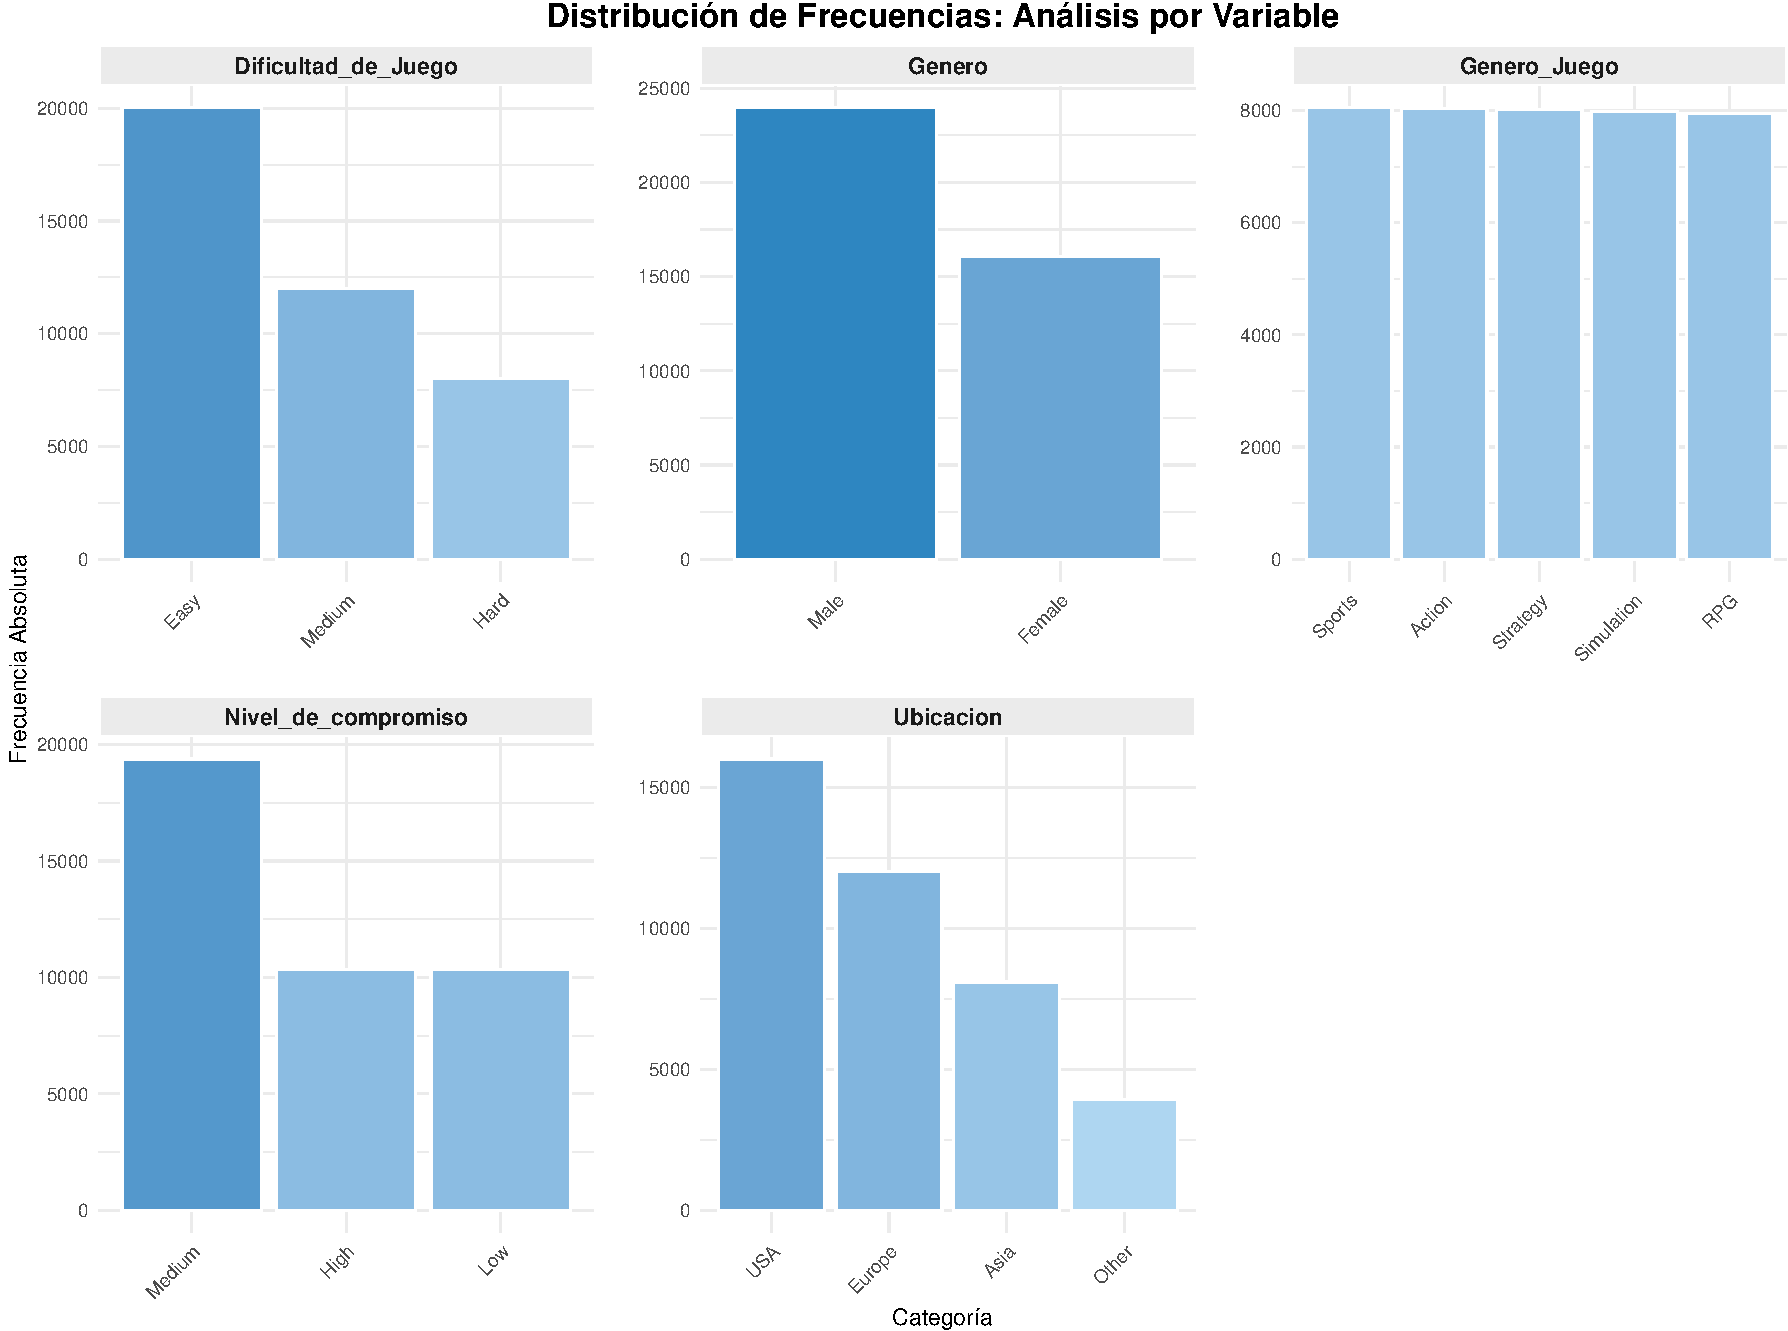
\includegraphics[width=0.9\linewidth,]{Análisis_del_comportamiento_de_los_jugadores_en_línea_Grupo_7_files/figure-latex/grafica_frecuencias_libres-1} \end{center}

Al observar el conjunto de resultados, tanto de las variables
cualitativas como de las cuantitativas, se puede ver que:\\

La edad promedio de 31.99 años revela una comunidad de adultos jóvenes.
En cuanto a la progresión, los jugadores se sitúan en un punto medio de
su experiencia dentro del juego con un nivel promedio de 49.66, lo que
indica que el sistema logra retener a los usuarios de manera efectiva,
permitiéndoles disfrutar de aproximadamente la mitad del contenido total
disponible antes de cualquier posible abandono.\\

Por otro lado, la preferencia mayoritaria por la dificultad ``Easy'' y
un compromiso de nivel ``Medium'' sugiere que el público objetivo busca
principalmente una forma de entretenimiento ligero. Finalmente, el hecho
de que el mayor volumen de datos provenga de USA y Europa evidencia una
clara tendencia marcada por los mercados occidentales.

\subsection{Limpieza de datos}

Para asegurar que el análisis sea confiable, se realizó un proceso de
depuración sobre el dataset original:

\begin{itemize}
  \item{Tratamiento de Valores Nulos (NAs): Se identificaron los valores ausentes para asegurar que los cálculos de correlación se realicen sobre pares completos de datos, evitando sesgos en los estimadores. Lo que dio por resultado que el dataset no presenta valores nulos.} 
  \item{Detección de Duplicados e Inconsistencias: Se detectaron registros redundantes y de sintaxis o tipos de datos inconsistentes que dificultarían la lectura por parte de los algoritmos de R. El resultado fue que el dataset no presenta duplicados ni inconsistencias.} 
  \item{Normalización de Variables: Se verificó que las variables numéricas mantuvieran una estructura coherente para facilitar el cálculo de los momentos centrales y los estadísticos de dispersión. Se obtuvo que el dataset no necesita normalización de variables ya que estas cumplen con la sintaxis necesaria.}
  \item{Detección de Valores Atípicos: Se verifico que no hubiera valores atípicos que afecten la media. Lo que dio por resultado que la variable Compras en el Juego contiene 8041 valores atípicos, ya que es una variable que no se toma en cuenta en la investigación no afecta el análisis.}
\end{itemize}

\chapter{Análisis de Resultados}

A continuación, se reportan los resultados del estudio, comenzando con
una descripción estadística exhaustiva de las variables. Posteriormente,
se añade el análisis de los resultados obtenidos.

\section{Géneros más populares por Ubicación}

A partir del primer objetivo de esta investigación (Identificar cuáles
son los géneros de juego más populares en cada ubicación), se presenta
la siguiente gráfica de barras agrupadas:

\begin{figure}[H]

{\centering 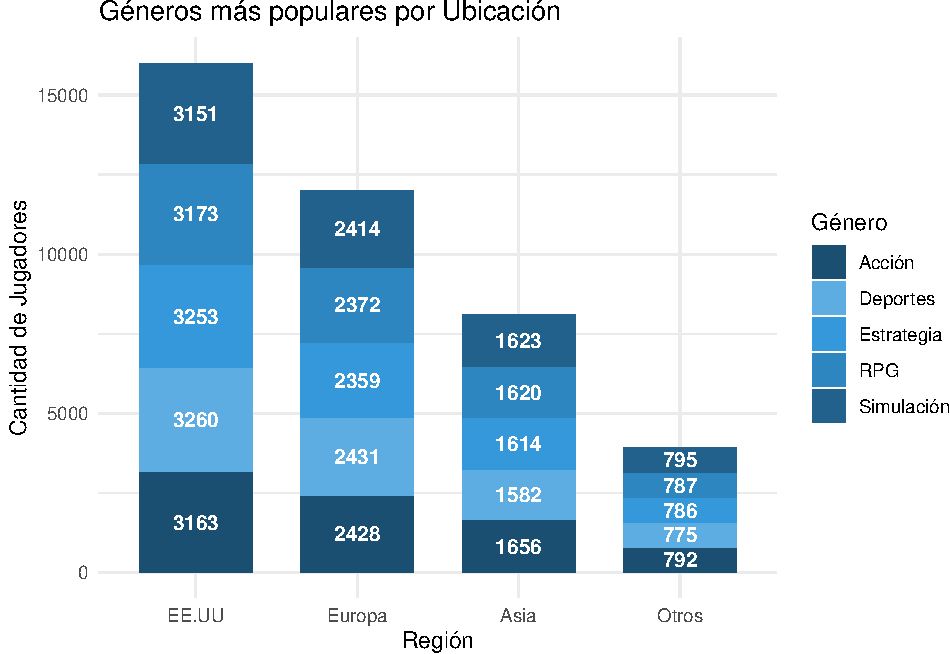
\includegraphics[width=0.8\linewidth,height=0.3\textheight,]{Análisis_del_comportamiento_de_los_jugadores_en_línea_Grupo_7_files/figure-latex/grafico-popularidad-1} 

}

\caption{Popularidad de Géneros por Ubicación}\label{fig:grafico-popularidad}
\end{figure}

Al observar las barras de manera individual, es posible identificar el
género predominante en cada ubicación (la barra de mayor altura):

\begin{itemize} 
  \item En EE.UU, se observa un ligero liderazgo del género Deportes (3,260). 
  \item En Europa, el género con mayor frecuencia es Deportes (2,431). 
  \item En Asia, destaca levemente el género Acción (1,656). 
  \item En la categoría Otros, la distribución es casi idéntica, con una mínima ventaja para Simulación (795). 
\end{itemize}

El análisis de popularidad permitió cumplir el objetivo de identificar
la moda estadística por región, determinando que en EE.UU y Europa
predomina el género de Sports, mientras que en Asia el liderazgo recae
en los videojuegos de Acción. No obstante, el hallazgo más relevante
para el contexto del mercado es la estrecha competitividad entre
categorías; la diferencia entre el género más popular y el menos
frecuente es mínima en todos los territorios, lo que define un mercado
globalizado y altamente diversificado donde ningún género ejerce un
monopolio de preferencia claro.

\section{Horas de Juego}

Para evaluar la distribución de las horas de juego, se presenta a
continuación un diagrama de caja (boxplot) que segmenta la variable
PlayTimeHours en tres niveles de dedicación:

\begin{figure}[H]

{\centering 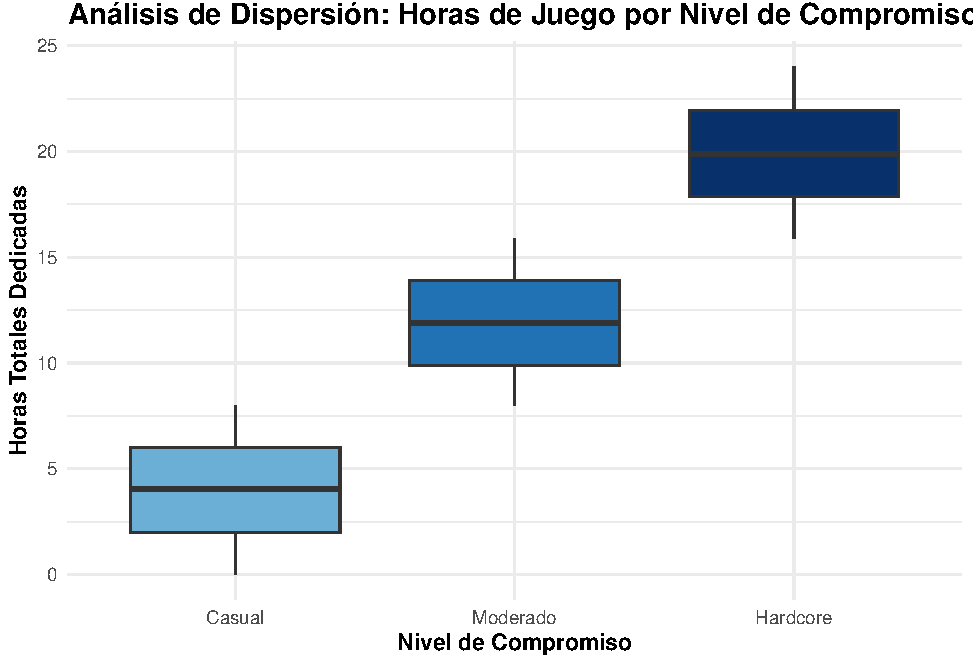
\includegraphics[width=0.85\linewidth,]{Análisis_del_comportamiento_de_los_jugadores_en_línea_Grupo_7_files/figure-latex/boxplot-compromiso-final-1} 

}

\caption{Distribución de Horas por Nivel de Compromiso}\label{fig:boxplot-compromiso-final}
\end{figure}

Al observar el gráfico, se nota que las categorías de Casual, Moderado y
Hardcore no se mezclan entre sí, lo que significa que cada tipo de
jugador tiene un hábito de consumo muy marcado y diferente al resto.
Mientras que los jugadores casuales son más constantes y predecibles en
sus pocas horas de juego, los jugadores ``Hardcore'' muestran una mayor
variedad, con algunos dedicando mucho más tiempo que otros dentro de su
misma categoría. Esta clara ``escalera'' en los niveles de dedicación
confirma que el mercado está segmentado por el grado de compromiso,
demostrando que la intensidad con la que se juega es un factor
determinante que diferencia a un perfil de otro.

\section{Comparación de las horas de dedicación entre frecuencia de sesiones semanales según distintos géneros de videojuegos.}

Para profundizar en la dinámica de uso, se presenta un análisis
comparativo que cruza la frecuencia de sesiones con el tiempo total de
juego, segmentado por cada género de videojuego:

\begingroup\fontsize{9}{11}\selectfont

\begin{longtable}[t]{>{\raggedright\arraybackslash}p{2.5cm}lrrr>{}l}
\caption{\label{tab:tabla-con-correlacion}Estadísticos de Dedicación y Coeficiente de Correlación por Género}\\
\toprule
Género & Rango Sesiones & Media & Mediana & Desv. Est. & Corr. Pearson (r)\\
\midrule
\endfirsthead
\caption[]{Estadísticos de Dedicación y Coeficiente de Correlación por Género \textit{(continued)}}\\
\toprule
Género & Rango Sesiones & Media & Mediana & Desv. Est. & Corr. Pearson (r)\\
\midrule
\endhead

\endfoot
\bottomrule
\endlastfoot
\textbf{\cellcolor{gray!10}{Acción}} & \cellcolor{gray!10}{0-5} & \cellcolor{gray!10}{12.26} & \cellcolor{gray!10}{12.42} & \cellcolor{gray!10}{6.83} & \textcolor{blue}{\em{\cellcolor{gray!10}{-0.011}}}\\
\textbf{} & 6-10 & 12.11 & 12.25 & 6.82 & \textcolor{blue}{\em{}}\\
\textbf{\cellcolor{gray!10}{}} & \cellcolor{gray!10}{11-15} & \cellcolor{gray!10}{12.17} & \cellcolor{gray!10}{12.30} & \cellcolor{gray!10}{6.97} & \textcolor{blue}{\em{\cellcolor{gray!10}{}}}\\
\textbf{} & 16-20 & 12.08 & 11.98 & 6.92 & \textcolor{blue}{\em{}}\\
\textbf{\cellcolor{gray!10}{Deportes}} & \cellcolor{gray!10}{0-5} & \cellcolor{gray!10}{12.00} & \cellcolor{gray!10}{11.94} & \cellcolor{gray!10}{6.90} & \textcolor{blue}{\em{\cellcolor{gray!10}{-0.005}}}\\
\addlinespace
\textbf{} & 6-10 & 11.98 & 12.14 & 6.94 & \textcolor{blue}{\em{}}\\
\textbf{\cellcolor{gray!10}{}} & \cellcolor{gray!10}{11-15} & \cellcolor{gray!10}{11.98} & \cellcolor{gray!10}{12.03} & \cellcolor{gray!10}{7.01} & \textcolor{blue}{\em{\cellcolor{gray!10}{}}}\\
\textbf{} & 16-20 & 11.88 & 11.49 & 6.93 & \textcolor{blue}{\em{}}\\
\textbf{\cellcolor{gray!10}{Estrategia}} & \cellcolor{gray!10}{0-5} & \cellcolor{gray!10}{11.73} & \cellcolor{gray!10}{11.45} & \cellcolor{gray!10}{6.93} & \textcolor{blue}{\em{\cellcolor{gray!10}{0.03}}}\\
\textbf{} & 6-10 & 12.20 & 12.54 & 6.98 & \textcolor{blue}{\em{}}\\
\addlinespace
\textbf{\cellcolor{gray!10}{}} & \cellcolor{gray!10}{11-15} & \cellcolor{gray!10}{12.17} & \cellcolor{gray!10}{12.26} & \cellcolor{gray!10}{6.90} & \textcolor{blue}{\em{\cellcolor{gray!10}{}}}\\
\textbf{} & 16-20 & 12.35 & 12.39 & 6.94 & \textcolor{blue}{\em{}}\\
\textbf{\cellcolor{gray!10}{RPG}} & \cellcolor{gray!10}{0-5} & \cellcolor{gray!10}{12.13} & \cellcolor{gray!10}{12.34} & \cellcolor{gray!10}{6.96} & \textcolor{blue}{\em{\cellcolor{gray!10}{-0.015}}}\\
\textbf{} & 6-10 & 11.98 & 11.79 & 6.87 & \textcolor{blue}{\em{}}\\
\textbf{\cellcolor{gray!10}{}} & \cellcolor{gray!10}{11-15} & \cellcolor{gray!10}{12.04} & \cellcolor{gray!10}{11.98} & \cellcolor{gray!10}{6.91} & \textcolor{blue}{\em{\cellcolor{gray!10}{}}}\\
\addlinespace
\textbf{} & 16-20 & 11.81 & 11.61 & 6.92 & \textcolor{blue}{\em{}}\\
\textbf{\cellcolor{gray!10}{Simulación}} & \cellcolor{gray!10}{0-5} & \cellcolor{gray!10}{12.12} & \cellcolor{gray!10}{12.12} & \cellcolor{gray!10}{6.78} & \textcolor{blue}{\em{\cellcolor{gray!10}{-0.017}}}\\
\textbf{} & 6-10 & 11.85 & 11.82 & 7.09 & \textcolor{blue}{\em{}}\\
\textbf{\cellcolor{gray!10}{}} & \cellcolor{gray!10}{11-15} & \cellcolor{gray!10}{11.66} & \cellcolor{gray!10}{11.46} & \cellcolor{gray!10}{6.82} & \textcolor{blue}{\em{\cellcolor{gray!10}{}}}\\
\textbf{} & 16-20 & 11.90 & 11.88 & 6.89 & \textcolor{blue}{\em{}}\\*
\end{longtable}
\endgroup{}

\textbf{Gráfico}

\begin{figure}[H]

{\centering 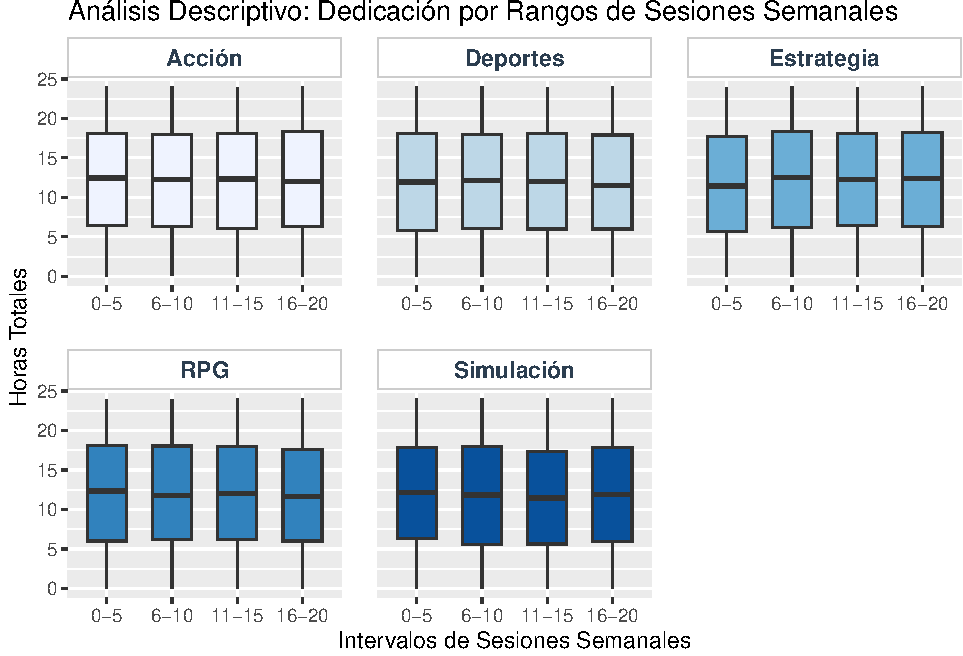
\includegraphics[width=1\linewidth,]{Análisis_del_comportamiento_de_los_jugadores_en_línea_Grupo_7_files/figure-latex/comparativa-interaccion-1} 

}

\caption{Distribución de Horas vs. Sesiones por Género}\label{fig:comparativa-interaccion}
\end{figure}

El análisis comparativo entre las horas totales de juego y la frecuencia
de sesiones semanales permite identificar el comportamiento de consumo
del usuario según el género del videojuego. Al observar la estabilidad
de las medianas y la distribución de los boxplots en todos los rangos se
puede ver el tiempo total de juego semanal se mantiene constante en un
promedio de 12 horas, independientemente de qué tan frecuente sea el
acceso del usuario o el género del videojuego. Los coeficientes de
correlación de Pearson obtenidos (aproximadamente 0) confirman la
ausencia de una relación lineal entre estas variables, lo que demuestra
que una mayor frecuencia de sesiones no se traduce en una mayor
dedicación horaria. Este fenómeno sugiere un comportamiento de
compensación, donde los jugadores ajustan la duración de sus partidas
según su disponibilidad: quienes entran pocas veces realizan sesiones
largas, mientras que los jugadores recurrentes optan por sesiones
breves.

\section{Relacion lineal entre Horas de Juego y Sesiones por Semana}

Para verificar si existe una relación directa entre el tiempo total de
juego y la constancia semanal, se procedió a calcular el Coeficiente de
Correlación de Pearson (r):

\begin{center}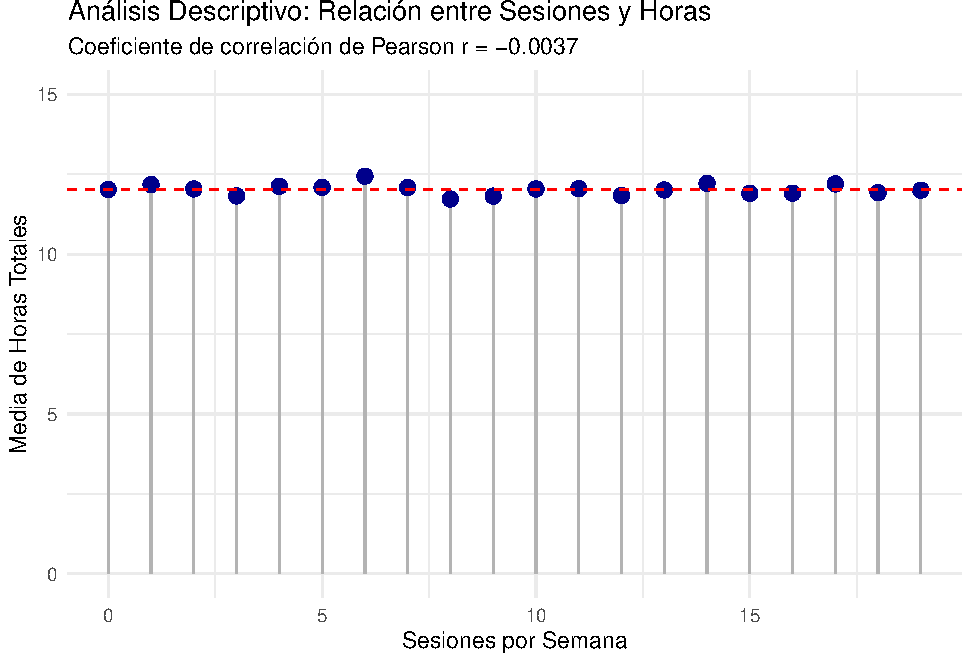
\includegraphics[width=0.9\linewidth,]{Análisis_del_comportamiento_de_los_jugadores_en_línea_Grupo_7_files/figure-latex/analisis-correlacion-definitivo-1} \end{center}

\begin{longtable}[t]{lll}
\caption{\label{tab:analisis-correlacion-definitivo}Resumen Estadístico de la Asociación Lineal}\\
\toprule
Metrica & Valor & Relacion\\
\midrule
Coeficiente de Pearson (r) & -0.0037 & Nula / Independiente\\
\bottomrule
\end{longtable}

Visualmente, se observa que los promedios de horas totales se mantienen
estables en todos los niveles de sesiones por semana. La trayectoria de
los puntos no presenta una dirección ascendente ni descendente,
situándose de forma persistente alrededor de las 12 horas. Aunque
existen ligeras variaciones donde algunos puntos se posicionan levemente
por encima o por debajo de la media general, estas oscilaciones son
marginales y no siguen un patrón de crecimiento. Esto describe una
homogeneidad en el consumo de tiempo, independientemente de la
constancia del usuario. Como medida resumen de la asociación lineal, se
obtuvo un valor de Correlación (aproximadamente 0). Al ser un valor
prácticamente nulo, actúa como evidencia de que no existe una relación
lineal entre ambas variables.

\chapter{Conclusiones y Recomendaciones}

\textbf{1.-} Conclusión 1: A través del análisis de las frecuencias de
géneros de videojuego por locación, se concluye que el mercado de
videojuegos es altamente homogéneo. Aunque se detectaron preferencias
ligeras, la diferencia con los demás géneros es tan pequeña que no se
puede hablar de un dominio absoluto. Esto sugiere que los gustos de los
jugadores se han globalizado, permitiendo que un mismo título tenga
potencial de éxito casi idéntico en cualquier continente.\\

\textbf{Recomendación:} Debido a que no existe un género que domine el
mercado de forma absoluta en ninguna región en los resultados de esta
investigación, existe una oportunidad para que las desarrolladoras se
arriesguen con nuevas propuestas. La paridad en los gustos globales
indica que el mercado está abierto a recibir cualquier género, siempre y
cuando la calidad del producto sea competitiva.\\

\textbf{2.-} Conclusion 2: Los datos muestran una separación clara y
ordenada en los niveles de consumo. Los jugadores no saltan de una
categoría a otra de forma aleatoria; se agrupan en tres perfiles bien
definidos:

\begin{itemize} 
  \item Casual: Constante y de bajo consumo. 
  \item Moderado: Un punto intermedio de compromiso.
  \item Hardcore: Un grupo más diverso, donde algunos llevan la dedicación al extremo. Esto nos indica que para predecir cuánto jugará alguien, es más importante saber qué tipo de jugador es que de qué país viene.
\end{itemize}

\textbf{Recomendación:} Al existir grupos tan definidos y sin cruces
entre sí, la estrategia debe abandonar el concepto de ``jugador
promedio'' y enfocarse en la especialización por nichos:

\begin{itemize} 
  \item Enfoque de Producto: Desarrollar mecánicas de entrada y salida rápida para el segmento Casual (baja dedicación/alta constancia) y sistemas de profundidad expansiva para el Hardcore (alta dedicación/alta variabilidad). 
  \item Eficiencia en la Inversión Publicitaria: Se recomienda redirigir los presupuestos de marketing hacia canales digitales que permitan segmentar por intereses y comportamientos de uso en lugar de límites geográficos. Al ser un mercado globalizado y competitivo, es más rentable captar a un "jugador de estrategia hardcore", en cualquier parte del mundo que intentar convencer a toda la población de una región específica. 
\end{itemize}

\textbf{3.-} Conclusion 3: Se concluye que no existe una regla general
que vincule la cantidad de veces que un usuario ingresa al juego con el
total de horas que le dedica. Los resultados reflejan que, sin importar
el género del videojuego, los hábitos de consumo son muy diversos.
Dentro de una misma categoría conviven de manera equilibrada jugadores
que prefieren conexiones diarias muy breves y aquellos que optan por
sesiones largas y esporádicas. Esto demuestra que la constancia semanal
y el volumen de tiempo invertido son decisiones personales del jugador,
independientes del tipo de videojuego que decida consumir.\\

\textbf{Recomendación: } Frente a esta variedad de perfiles, se sugiere
a los desarrolladores adoptar estrategias de retención más flexibles,
evitando diseñar sus productos pensando en un único tipo de consumidor.
Es recomendable crear sistemas de recompensas que valoren por igual los
accesos frecuentes y las sesiones prolongadas. Por ejemplo, en lugar de
ofrecer premios únicamente por ingresar todos los días, se deben incluir
incentivos por horas de juego acumuladas o metas a largo plazo. Así, el
producto se adapta orgánicamente a los diferentes estilos de vida de los
jugadores.\\

\textbf{3.-} Conclusion 4:\\
Se concluye que la frecuencia de sesiones por semana no es un indicador
del volumen total de tiempo invertido en el juego. El hallazgo de una
relación lineal nula entre estas variables demuestra que la constancia
(qué tan seguido se juega) y la dedicación (cuánto tiempo se juega en
total) son comportamientos totalmente independientes. Esto significa que
un jugador que ingresa muchas veces por semana no necesariamente acumula
más horas que alguien que ingresa pocas veces, pero en sesiones de larga
duración.\\

\textbf{Recomendación: } Se recomienda implementar una estrategia de
fidelización híbrida que reconozca la independencia entre la constancia
y la duración del juego; dado que un mayor número de sesiones no
garantiza un mayor tiempo total, los desarrolladores deben diseñar
incentivos diferenciados que premien por igual los accesos rápidos
diarios (micro-objetivos) y las sesiones de larga duración
(macro-objetivos). Este enfoque permite captar el valor de ambos
perfiles de usuario de forma aislada, optimizando la retención al
adaptar la oferta de contenido al estilo de vida específico de cada
jugador en lugar de aplicar un modelo de métricas unificado.

\appendix
\renewcommand{\thechapter}{\Alph{chapter}}

\chapter{Anexo A}

\begin{center}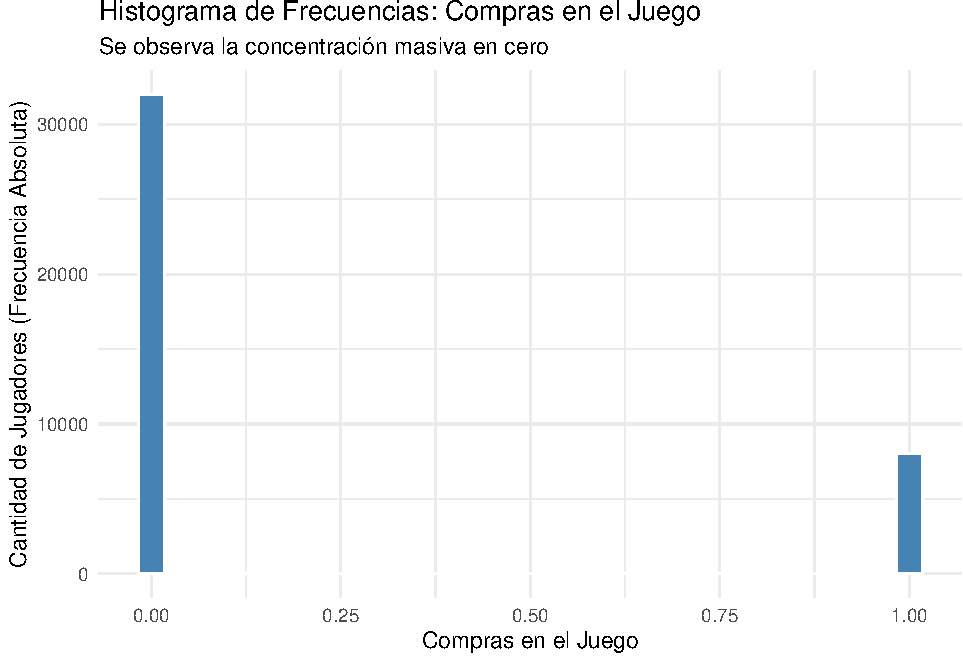
\includegraphics[width=0.9\linewidth,]{Análisis_del_comportamiento_de_los_jugadores_en_línea_Grupo_7_files/figure-latex/anexo-frecuencia-compras-1} \end{center}

Durante la fase de limpieza de los 40,000 datos, llamó la atención un
fenómeno particular con la variable Compras en el Juego. Al intentar
analizarla, el sistema detectó valores atípicos, lo que inicialmente
parecía un error, pero resultó ser un descubrimiento clave sobre el
comportamiento de los jugadores. Al graficar estos datos, se hizo
evidente que la muestra está dividida en dos grupos muy marcados: una
gran mayoría del 80\% de los jugadores que no realiza ninguna compra, y
un grupo específico del 20\% que sí lo hace.

\chapter{Anexo B}

\textbf{Validación de Calidad e Integridad de la Muestra}\\

Tras auditar los registros del dataset, se confirmó la ausencia total de
valores nulos y una alta consistencia en las categorías analizadas.
Llamó la atención la variabilidad que presenta la variable
Duración\_Promedio, cuya varianza de 2402.11 refleja la diversidad real
de los tiempos de juego, contrastando con la estabilidad del resto de
las métricas. Este control de calidad asegura que los resultados
presentados no son producto de errores de captura o datos atípicos
accidentales, sino que representan tendencias sólidas y fiables del
comportamiento de los usuarios en la muestra.

\chapter{Referencias Bibliográficas}

Hamari, J., \& Lehdonvirta, V. (2010). Game design as marketing: How
game mechanics create demand for virtual goods. \emph{International
Journal of Business Science \& Applied Management}, 5(1), 14-29.\\

Kapalo, K. A., Dixon, D., Murphy, R., \& Adams, D. (2015). Determining
Player Intensity: A Statistical Approach to Hardcore vs.~Casual
Profiles. \emph{International Journal of Human-Computer Interaction},
31(10), 655-667.\\

Newzoo. (2025). \emph{Global Games Market Report 2025}. Recuperado de
\url{https://newzoo.com}\\

Olagunju, T. (2026). Analysis of Regional Video Game Sales and Genre
Trends. \emph{Journal of Gaming Analytics}.\\

Pyramid Technologies. (2026). \emph{Understanding Stickiness and
Retention in Modern Gaming}. Tech Report.\\

ResearchGate. (2025). \emph{Predictive Modeling of Player Engagement by
Game Genre}. Gaming Insights Series.\\

Statista. (2025). \emph{Video Game Demographics and Geographic Usage
Patterns}. Recuperado de \url{https://www.statista.com}\\

Tilburg University. (2023). \emph{Cultural Influence on Gaming Styles
and Player Behavior}. Academic Repository.\\

Vertica. (2024). \emph{Data-Driven Competitive Advantage in the Gaming
Industry}. White Paper.\\

Webster, J. G. (2014). \emph{The Marketplace of Attention: How Audiences
Take Shape in a Digital Age}. MIT Press.\\

El Kharoua, R. (2024). Predict Online Gaming Behavior Dataset
{[}Conjunto de datos{]}. Kaggle.
\url{https://www.kaggle.com/datasets/rabieelkharoua/predict-online-gaming-behavior-dataset}\\

%%%%%%%%%%%%%%%%%%%%%%%%%%%%%%%%%%%%%%%%%%%%%%%%%%%%%
%                   REFERENCIAS                     %
%%%%%%%%%%%%%%%%%%%%%%%%%%%%%%%%%%%%%%%%%%%%%%%%%%%%%
% Mantenemos la estructura natbib de tu plantilla
\renewcommand{\bibname}{Lista de Referencias}
\bibliographystyle{apalike} 
\bibliography{bibliografia.bib} 

%%%%%%%%%%%%%%%%%%%%%%%%%%%%%%%%%%%%%%%%%%%%%%%%%%%%%
%                   APÉNDICES                       %
%%%%%%%%%%%%%%%%%%%%%%%%%%%%%%%%%%%%%%%%%%%%%%%%%%%%%

\end{document}
